\documentclass[10pt,twocolumn,a4paper]{ctexart}
\usepackage[margin=1.7cm,columnsep=0.65cm]{geometry}
\usepackage{amsmath,amssymb,bm}
\usepackage{booktabs,multirow}
\usepackage{graphicx}
\usepackage{microtype}
\usepackage{natbib}
\usepackage{xcolor}
\usepackage{hyperref}
\usepackage{enumitem}
\usepackage{fancyhdr}
\usepackage{listings}

\graphicspath{{../../artifacts/figures/}}
\setlength{\parindent}{2em}
\setlist{nosep,leftmargin=*}
\hypersetup{colorlinks=true,linkcolor=blue!55!black,
  citecolor=green!45!black,urlcolor=blue!65!black}
\pagestyle{fancy}
\fancyhf{}
\fancyhead[L]{Imitation Learning Interview Guide}
\fancyhead[R]{ShaneLiu04}
\fancyfoot[C]{\thepage}
\lstset{basicstyle=\ttfamily\footnotesize,breaklines=true,
  frame=single,columns=fullflexible}

\providecommand{\BCEasyMean}{--}
\providecommand{\BCEasyStd}{--}
\providecommand{\BCHardMean}{--}
\providecommand{\BCHardStd}{--}
\providecommand{\FlowHardMean}{--}
\providecommand{\FlowHardStd}{--}
\providecommand{\DaggerHardMean}{--}
\providecommand{\DaggerHardStd}{--}
\providecommand{\NumSeeds}{--}
\providecommand{\GPUName}{NVIDIA RTX 6000D}
\InputIfFileExists{../results_macros.tex}{}{}

\title{\vspace{-1.2em}\textbf{从 Behavior Cloning 到生成式策略：\\
面向算法、机器人与强化学习面试的模仿学习知识体系}}
\author{ShaneLiu04\\
\small\url{https://github.com/ShaneLiu04}}
\date{}

\begin{document}
\maketitle
\thispagestyle{fancy}

\begin{abstract}
本文围绕求职面试中常见的“从示范学习策略”问题，建立从统计学习、序列决策到系统实现的
统一框架。内容以一个可复现的 Flappy Bird Assignment 为贯穿案例，解释 Behavior
Cloning 的最大似然视角、compounding error、multimodal action、Flow Matching、
DAgger、action chunking 及闭环评测，并延伸到 Diffusion Policy、Behavior
Transformer、Implicit BC、GAIL 和 Vision-Language-Action 模型。与只罗列算法不同，
本文强调四种能力：现场推导、接口实现、实验诊断与研究判断。每个主题均给出面试回答骨架、
常见误区和可落地的工程检查项。
\end{abstract}

\textbf{关键词：}求职面试；Imitation Learning；Generative Policy；
Distribution Shift；Robot Learning；Experimental Methodology

\section{统一视角：模仿学习究竟在学什么}
设有限时域 MDP
$\mathcal M=(\mathcal S,\mathcal A,P,r,\rho_0,T)$，专家策略为 $\pi_E$。
模仿学习获得专家示范
$\mathcal D=\{\tau_i\}$，其中
$\tau=(s_0,a_0,\ldots,s_T)$，目标是学得策略 $\pi_\theta$，使其在环境中的访问分布和
性能接近专家。与普通 supervised learning 的关键差别是：分类器的预测通常不改变下一条
输入，而控制策略的动作会通过 $P(s_{t+1}\mid s_t,a_t)$ 改变未来输入。

面试时可以先给出三层分解：
\begin{enumerate}
  \item \textbf{输出建模：}对给定状态，动作是单峰、多峰还是结构化序列；
  \item \textbf{访问分布：}训练状态来自专家 $d_{\pi_E}$，部署状态来自策略
  $d_{\pi_\theta}$；
  \item \textbf{闭环系统：}动作频率、延迟、horizon 和安全约束决定模型如何落地。
\end{enumerate}
BC、Flow Matching 与 DAgger 分别主要解决上述前两层的不同部分。

\section{Behavior Cloning 的统计本质}
\subsection{离散动作与连续动作}
离散动作 BC 常写为负对数似然
\[
  \mathcal L(\theta)=-\mathbb E_{(s,a)\sim\mathcal D}
  [\log\pi_\theta(a\mid s)].
\]
若连续动作策略设为固定方差 Gaussian，
$\pi_\theta(a\mid s)=\mathcal N(\mu_\theta(s),\sigma^2I)$，最大似然等价于 MSE：
\[
  -\log\pi_\theta(a\mid s)=
  \frac{1}{2\sigma^2}\|a-\mu_\theta(s)\|_2^2+C.
\]
因此 MSE 并非任意选择，它隐含“条件动作近似单峰 Gaussian 且各维同方差”的假设。

\subsection{为什么多峰动作会被平均}
对固定 $s$，最小化
$\mathbb E[\|f(s)-a\|_2^2\mid s]$。对 $f$ 求导并令其为零：
\[
  2(f(s)-\mathbb E[a\mid s])=0
  \Rightarrow f^\star(s)=\mathbb E[a\mid s].
\]
若绕障碍物向左、向右都正确，均值可能径直撞向障碍物。Flappy Bird hard expert 在两个
缺口之间随机选择，图~\ref{fig:modes-guide} 直观展示这一点。

\begin{figure}[t]
  \centering
  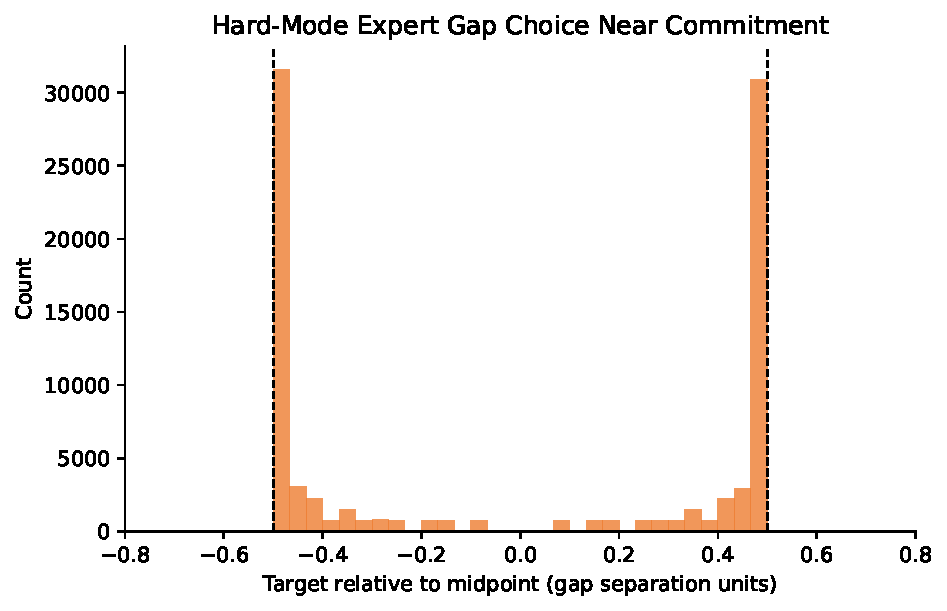
\includegraphics[width=\columnwidth]{hard_action_distribution}
  \caption{hard expert 的多峰动作。MSE 最优解位于两峰之间。}
  \label{fig:modes-guide}
\end{figure}

\subsection{面试回答模板}
\textbf{问题：BC 的优缺点是什么？}
\begin{itemize}
  \item 优点：目标稳定、无需 reward、训练可并行、可复用监督学习基础设施；
  \item 局限：covariate shift、compounding error、多峰均值化、示范质量上限；
  \item 诊断：同时看 validation NLL/MSE 和 closed-loop rollout，不用低 loss 代替任务成功；
  \item 改进：数据增强/重加权、mixture density、latent-variable/generative policy、
  DAgger 或 offline RL。
\end{itemize}

\section{Compounding Error：从单步误差到轨迹失败}
设策略在专家状态分布上的单步错误率不超过 $\epsilon$。一旦出错，策略可能进入训练未覆盖
区域，后续每一步都更易出错。朴素 worst-case 分析可得到总成本差距
$O(T^2\epsilon)$；在额外稳定性假设下可更紧，但核心是状态分布由过去动作内生决定。
\citet{ross2010efficient,ross2011dagger} 将此问题转化为 no-regret online learning，
DAgger 可把依赖改善到 $O(T\epsilon)$ 量级。

\textbf{现场解释。}不要只说“误差会累积”。应明确因果链：
\[
\begin{aligned}
\text{action error}&\rightarrow\text{off-expert state}\\
&\rightarrow\text{no training support}\rightarrow\text{larger error}.
\end{aligned}
\]
这也解释了为什么随机打乱 train/test transitions 可能产生乐观估计：两个集合仍来自同一
expert occupancy，而真正部署考验的是 policy occupancy。

\section{DAgger：数据闭环而不是模型技巧}
\subsection{算法}
DAgger 初始化 $\mathcal D_0$ 为专家数据。第 $i$ 轮执行混合策略或当前策略，收集访问状态，
查询专家标签并聚合：
\[
  \mathcal D_i=\mathcal D_{i-1}\cup
  \{(s,\pi_E(s)):s\sim d_{\pi_i}\}.
\]
再在 $\mathcal D_i$ 上训练 $\pi_{i+1}$。关键词是 \textbf{aggregate}；只保留最新一轮会
导致 catastrophic forgetting。理论上混合专家可以提高早期安全性，实践中 $\beta_i$
逐轮衰减。

\subsection{工程难点}
\begin{enumerate}
  \item \textbf{专家可查询性：}人类、规划器或规则控制器能否对任意访问状态给标签；
  \item \textbf{安全性：}差策略是否允许上线采集，是否需要 shield 或 simulation；
  \item \textbf{标签一致性：}随机专家可能给近邻状态冲突标签；
  \item \textbf{数据权重：}早期大规模专家数据可能淹没后期关键纠错状态；
  \item \textbf{checkpoint：}DAgger 曲线可能非单调，应基于独立 rollout 选择模型。
\end{enumerate}

\begin{figure}[t]
  \centering
  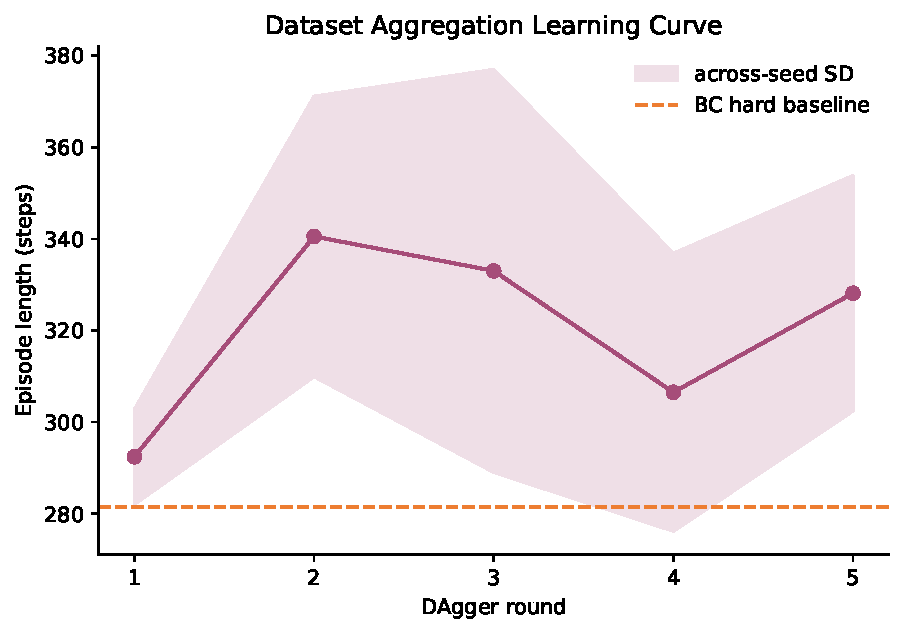
\includegraphics[width=\columnwidth]{dagger_learning_curve}
  \caption{DAgger 的经验学习曲线，用于讨论分布覆盖和跨 seed 方差。}
\end{figure}

\textbf{问题：DAgger 和 online RL 有何区别？}DAgger 的监督信号来自专家动作，通常不需要
reward 或 credit assignment；online RL 从环境回报优化策略，可超越专家但方差和样本
复杂度更高。二者都改变数据收集分布，但 oracle 和优化目标不同。

\section{多模态策略建模工具箱}
\subsection{Mixture Density Network}
用
$p(a\mid s)=\sum_{k=1}^{K}\alpha_k(s)\mathcal N(a;\mu_k(s),\Sigma_k(s))$
显式表示有限个模式。优点是 likelihood 清晰、单次前向速度快；难点是 mode 数需预设、
训练可能 component collapse，且高维 action chunk 的 full covariance 昂贵。

\subsection{Behavior Transformer}
Behavior Transformer 先对动作序列聚类或离散化，再由 Transformer 预测 mode token 和
连续 residual\citep{shafiullah2022bet}。它把“选择哪一种行为”和“模式内精修”分开，
适合长序列和多模态示范，但 tokenization 质量成为新的瓶颈。

\subsection{Implicit Behavioral Cloning}
IBC 学习能量函数 $E_\theta(s,a)$，通过 contrastive objective 让专家动作具有低能量，
推理时优化或采样
$\arg\min_a E_\theta(s,a)$\citep{florence2022implicit}。能量模型可以表达复杂分布，
代价是 action optimization 的延迟与稳定性。

\subsection{Diffusion 与 Flow Matching}
Diffusion Policy 用逐步去噪生成 action sequence，在多个机器人任务上展示多模态和时间
一致性\citep{chi2023diffusion}。Flow Matching 直接回归概率路径的 velocity field：
\[
x_t=(1-t)x_0+tx_1,\qquad u_t=x_1-x_0,
\]
\[
\mathcal L_{\rm FM}=\mathbb E\|v_\theta(x_t,s,t)-u_t\|^2.
\]
它的训练不需要对 ODE solver 反向传播；推理成本由函数评估次数 NFE 决定。面试时应说明
“生成式”不是目的，只有当 $p(a\mid s)$ 多峰或序列相关时，额外计算才可能带来收益。

\section{Flow Matching 推导与实现检查}
\subsection{从 continuity equation 到采样}
时间相关密度 $p_t(x)$ 在向量场 $v_t(x)$ 下满足
\[
  \partial_t p_t(x)+\nabla\cdot(p_t(x)v_t(x))=0.
\]
若 learned field 与目标路径的 conditional vector field 在 MSE 意义下匹配，其边缘
field 可输运 $p_0$ 到数据分布 $p_1$\citep{lipman2023flow}。采样求解 ODE
$dx/dt=v_\theta(x,s,t)$。一阶 Euler 为
$x_{k+1}=x_k+\Delta t\,v_\theta(x_k,s,t_k)$。

\subsection{高频实现错误}
\begin{itemize}
  \item 把 velocity 写成 $x_0-x_1$，导致采样方向反转；
  \item $t$ shape 为 $(B,)$，没有扩展到 action 的额外维度；
  \item Euler step 使用 $S$ 而不是 $1/S$；
  \item 训练与推理的时间参数范围或 dtype 不一致；
  \item 忘记 sample 使用 \texttt{no\_grad}，产生无意义计算图；
  \item 只看 velocity MSE，不做闭环 rollout 和 sampler steps 消融。
\end{itemize}

\begin{figure}[t]
  \centering
  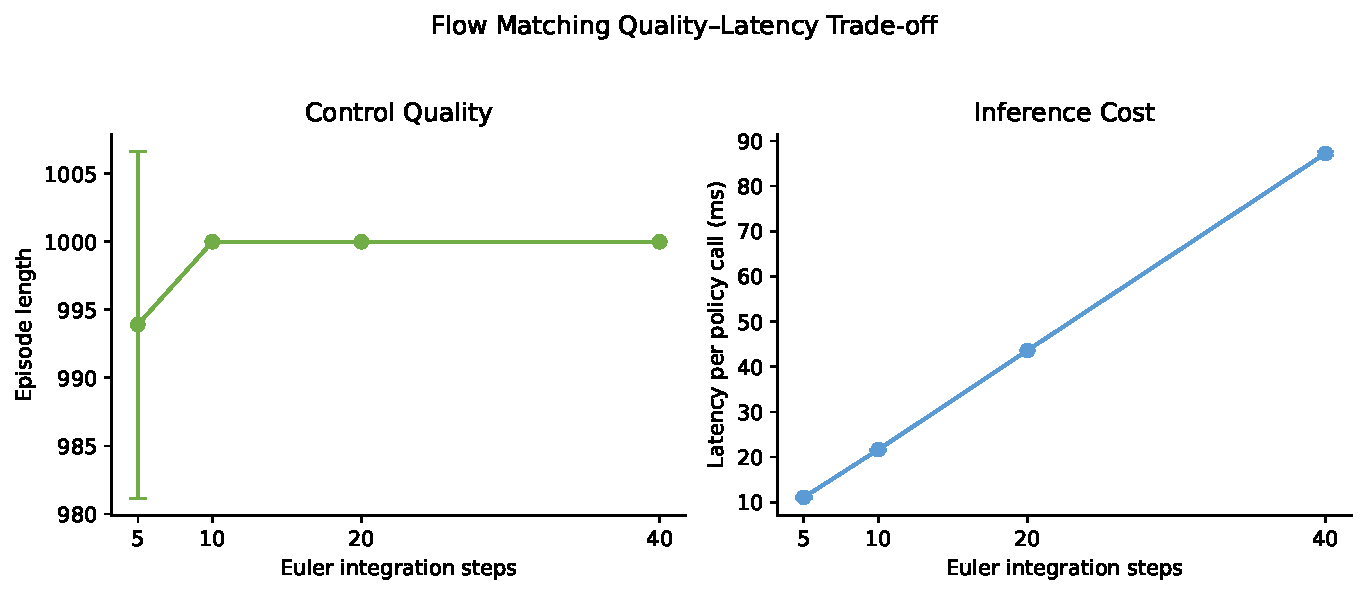
\includegraphics[width=\columnwidth]{flow_steps_ablation}
  \caption{NFE 对控制质量与延迟的影响。部署需要寻找 Pareto 点。}
\end{figure}

\section{Action Chunking 与系统设计}
逐步动作策略每个环境 step 查询一次模型，反馈快但 latency 高，且相邻输出可能抖动。
action chunking 预测
$\bm a_{t:t+H-1}$，利用序列模型学习时间相关性。ACT 在低成本双臂操作中结合
Transformer 与 action chunking\citep{zhao2023act}。

部署时还要定义执行长度 $K\le H$：
\begin{itemize}
  \item $K=1$：反馈最强，推理请求最多；
  \item $K=H$：吞吐最好，但完全开环；
  \item $1<K<H$：receding horizon，每 $K$ 步根据新观测重规划。
\end{itemize}
若推理耗时为 $t_{\rm infer}$，控制周期为 $\Delta t$，实时约束近似为
$t_{\rm infer}\le K\Delta t$。但增大 $K$ 不是免费加速，它会放大模型误差和外部扰动。

\begin{figure}[t]
  \centering
  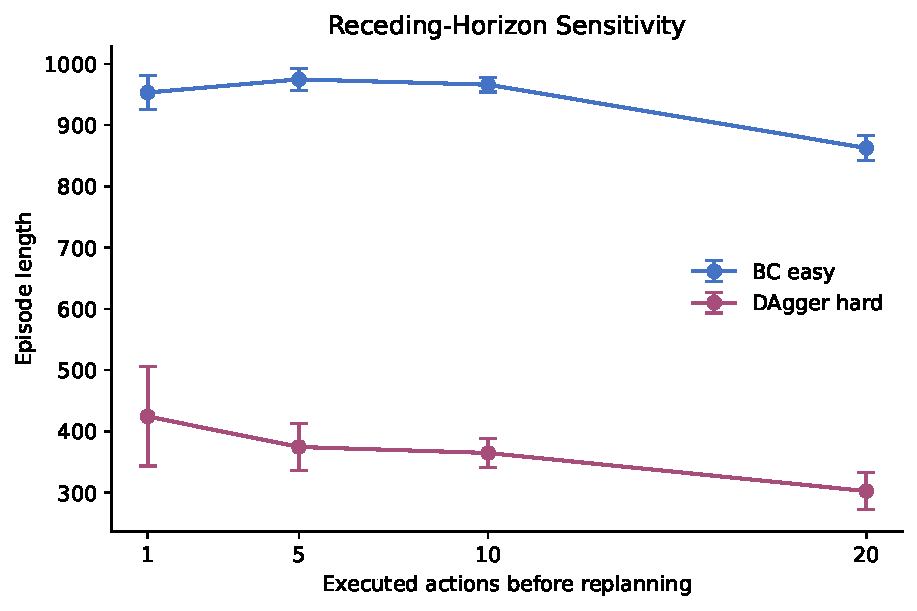
\includegraphics[width=\columnwidth]{execute_steps_ablation}
  \caption{重规划频率消融。报告 action horizon 时必须同时报告 $K$。}
\end{figure}

\section{评测：如何避免“漂亮但无效”的实验}
\subsection{统计单元与随机种子}
控制任务的独立统计单元是 episode，而不是 transition。训练使用多个 seed 是为了估计算法
对初始化、采样和环境随机性的稳定性。推荐同时报告：
\[
\begin{aligned}
  &\text{mean}\pm\text{SD},\quad\text{median},\quad\text{success rate},\\
  &n_{\rm seeds},\quad n_{\rm episodes}.
\end{aligned}
\]
不同方法应共享 evaluation seeds，以降低环境难度差异带来的方差；训练 seed 与评价 seed
应分离。

\subsection{数据泄漏与公平比较}
\begin{itemize}
  \item 同一轨迹的相邻窗口高度相关，不能随机拆成 train/test 后宣称泛化；
  \item 调参使用 validation seeds，最终 test seeds 只运行一次；
  \item 比较生成模型时同时给出 NFE、latency、参数量和训练预算；
  \item DAgger 使用更多专家查询，表格中必须报告 query budget；
  \item 只比较最终 return 会掩盖 failure mode，应保留 episode-level raw metrics。
\end{itemize}

\subsection{图表应该回答什么}
主结果图回答“谁更好”；learning curve 回答“数据或计算增加时怎样变化”；ablation
回答“哪个组件导致改进”；failure histogram 回答“在哪里失败”；quality--latency 图回答
“部署代价是什么”。如果一张图不能对应一个明确 claim，它通常不值得消耗计算。

\section{调试框架：从 tensor 到闭环}
\subsection{第一层：接口与数值}
先用小 batch 检查 shape、dtype、device、输出范围、finite loss 和非空梯度。对 Flow
Matching 检查 $t=0$ 与 $t=1$ 端点；对 action chunk 检查 $(B,Hd_a)$ 与
$(B,H,d_a)$ reshape 顺序。固定 seed 后运行两次，应得到一致结果。

\subsection{第二层：过拟合小数据}
在 32--256 个样本上训练到接近零 loss。若失败，优先检查 optimizer、learning rate、
normalization 和标签对齐；此时不要启动完整训练。对序列窗口最常见的是 state $s_t$
配到了 $a_{t+1:t+H}$ 而不是 $a_{t:t+H-1}$。

\subsection{第三层：open-loop 与 closed-loop}
先评估 held-out action error，再执行短 horizon rollout，最后执行完整 episode。若
open-loop 好、closed-loop 差，检查 distribution shift、控制频率和动态稳定性，而不是
盲目扩大模型。若 expert 自身不能稳定成功，先修复 oracle 与环境接口。

\subsection{第四层：性能剖析}
小 MLP 往往受 Python/environment 限制而非 GPU FLOPS 限制。应测量 data collection、
host-to-device、training step、policy query 和 environment step，而不是只看
\texttt{nvidia-smi}。有统计价值的多 seed 并行通常优于无意义增大模型。

\section{研究脉络与方法选择}
\subsection{从 BC 到 occupancy matching}
GAIL 通过 adversarial objective 匹配 expert 与 policy occupancy measure
\citep{ho2016gail}，避免逐状态专家查询，但需要环境交互且训练可能不稳定。其核心区别是
BC 匹配 conditional action，GAIL 更接近匹配轨迹访问分布。面试中可用“是否有环境、
reward、专家 oracle”决定方法：
\begin{itemize}
  \item 只有静态示范：BC、generative BC、offline RL；
  \item 可交互且可查询专家：DAgger；
  \item 可交互但不可查询专家：GAIL/IRL 或 RL fine-tuning；
  \item 有高质量 reward：以 BC 初始化，再 online RL。
\end{itemize}

\subsection{从低维控制到机器人基础模型}
真实机器人数据具有视觉高维、跨 embodiment、动作异构和多任务条件。Open
X-Embodiment 汇集跨机器人数据并训练 RT-X 系列模型\citep{openx2024}，RT-2 将
web-scale vision-language 知识迁移到动作预测\citep{brohan2023rt2}。规模化并未消除本
文问题：多模态输出、数据覆盖、闭环延迟和评测泄漏仍然存在，只是发生在更高维空间。

\subsection{示范质量与数据策展}
机器人 BC 对 demonstration quality、观测信息、采集设备和任务覆盖高度敏感。
\citet{mandlekar2022matters} 系统讨论了 human demonstrations 中影响性能的因素。
工程实践中，新增 10\% 高价值 failure recovery data 可能优于新增 100\% 重复成功轨迹。
这与 DAgger 的思想一致：数据价值由它覆盖的 policy failure distribution 决定。

\section{系统设计题：一个可上线的模仿学习平台}
面试中的开放题可以按数据、训练、评价、部署、监控五层回答。

\textbf{数据层：}轨迹采用 immutable object storage，metadata 记录环境版本、传感器
校准、expert ID、任务、成功标签与 license；基于 episode 划分数据，支持 lineage 和
去重。\textbf{训练层：}配置版本化，分布式 data loader，多 seed job array，checkpoint
含模型、optimizer、normalizer 与 Git commit。\textbf{评价层：}固定 scenario bank，
离线指标和 simulation rollout 分层，真实设备用 canary budget。
\textbf{部署层：}导出模型后测 p50/p95 latency、warm-up、batch=1 和 memory；控制器设置
超时 fallback 与 action bounds。\textbf{监控层：}记录 state/action drift、intervention、
near-miss、成功率和模型版本，触发 targeted data collection。

\section{高频追问与高质量回答}
\subsection{为什么 BC 不需要 Bellman equation}
BC 直接拟合专家动作，不估计 return 或 value，也不做 temporal credit assignment。
轨迹的时间结构可以通过 observation history 或 action chunk 进入模型，但优化目标仍是
supervised likelihood。只有引入 reward/value 做策略改进时才需要 Bellman structure
\citep{sutton2018rl}。

\subsection{DAgger 一定优于 BC 吗}
不一定。若 expert query 昂贵、专家在 off-distribution state 上不可靠、在线访问不安全，
或原数据已充分覆盖部署分布，DAgger 的成本可能大于收益。回答应比较 oracle quality、
interaction budget 和 safety constraint，而不是只背理论界。

\subsection{Flow Matching 为什么比 MSE 适合多峰}
MSE 的 deterministic head 只能输出一个条件均值；Flow Matching 把随机初值通过条件
向量场映射到不同动作模式。关键不是 loss 名称，而是 policy family 从 delta/Gaussian
mean 扩展为可采样分布。若数据单峰，生成式模型可能只增加 latency。

\subsection{Diffusion 和 Flow Matching 如何选择}
比较四点：训练 target（noise/score vs velocity）、概率路径、sampler/NFE、现有工程
生态。两者都能生成多峰 action sequence；Flow Matching 的直线路径和 ODE 表述通常更
直接，Diffusion Policy 有更成熟的机器人经验。最终应在同一 architecture、data、
evaluation seed 和 latency budget 下比较。

\subsection{为什么要预测 action chunk}
它利用动作时间相关性，降低每步推理开销，并减少高频输出抖动。代价是执行期间对新观测
响应变慢，因此通常只执行 chunk 前缀并重规划。回答中同时提 $H$ 与 $K$，体现系统意识。

\subsection{如何判断失败来自模型还是数据}
建立证据链：expert ceiling；小数据过拟合；held-out supervised metric；state coverage；
closed-loop failure states；oracle relabel；模型容量/生成方式消融。若在 failure states
补少量标签即可恢复，主要是 coverage；若同一 state 有冲突动作，主要是 multimodality；
若训练集都拟合不了，再考虑优化或容量。

\section{本作业证据如何转化为面试故事}
可按 STAR 结构表达：
\begin{itemize}
  \item \textbf{Situation：}hard mode 的两个合法缺口导致多峰示范；
  \item \textbf{Task：}完成 BC、Flow Matching、DAgger，并建立可复现实验；
  \item \textbf{Action：}先写 shape/endpoint/gradient tests，再运行 \NumSeeds{} seeds；
  保存 episode-level JSON；做 sampler steps 和 execute steps 消融；
  \item \textbf{Result：}BC easy 为 \BCEasyMean{}，hard 降至 \BCHardMean{}；
  Flow 与 DAgger 分别达到 \FlowHardMean{} 和 \DaggerHardMean{}；
  \item \textbf{Reflection：}监督 loss 下降不等于闭环成功，方法选择应对应输出分布和访问
  分布，GPU 利用率也应服务于统计证据而不是表面占用率。
\end{itemize}
该故事同时体现算法推导、PyTorch 实现、远端实验、统计设计和技术写作能力。

\section{面试前自检清单}
\begin{itemize}
  \item 能从 Gaussian MLE 推导连续动作 MSE；
  \item 能解释 $O(T^2\epsilon)$ compounding error 的假设与直觉；
  \item 能写出 DAgger 伪代码并说明 aggregate、$\beta_i$ 与 oracle；
  \item 能写出 Flow Matching 的 interpolation、velocity target 和 Euler sampler；
  \item 能比较 MDN、BeT、IBC、Diffusion、Flow Matching 的表达力与延迟；
  \item 能解释 action horizon 与 execute steps 的区别；
  \item 能设计 episode-level、多 seed、共享评价场景的实验；
  \item 能提出 safety、latency、drift 和 failure recovery 的上线方案；
  \item 能指出“低 training loss”“GPU 满载”“单个最好 seed”为什么都不是充分证据。
\end{itemize}

\section{结语}
模仿学习的核心不只是把 expert action 当 label。高质量解法需要同时回答三个问题：
policy family 能否表达条件动作分布，训练数据是否覆盖 policy occupancy，部署闭环是否在
延迟与反馈约束下稳定。BC、生成式策略和 DAgger 分别提供不同工具。研究与工程能力的分界
不在于记住更多算法名称，而在于能否把 failure observation 转化为可证伪假设，再用最小
而有解释力的实验验证它。

\bibliographystyle{plainnat}
\bibliography{../references}
\end{document}
